% !TeX spellcheck = en_US
\chapter{Data Structures}

\section{Introduction}

\begin{center}
	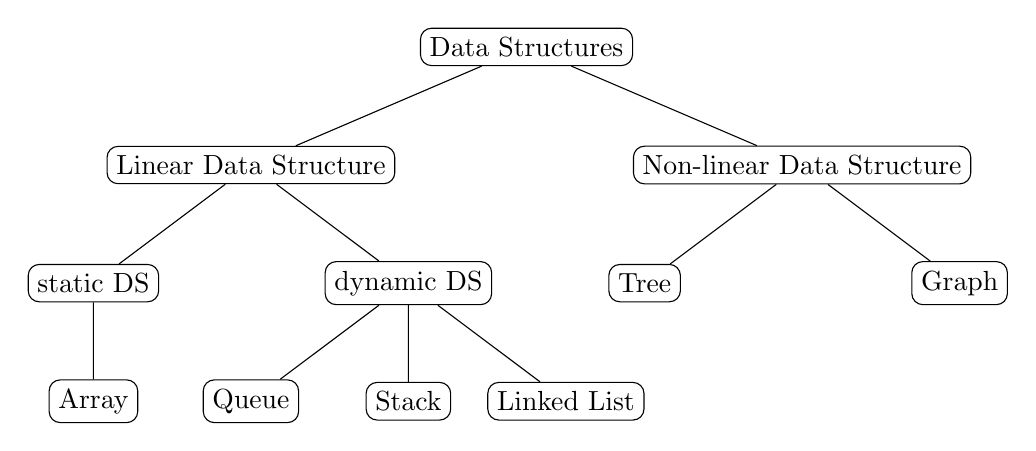
\begin{tikzpicture}[sibling distance=10em,
		every node/.style = {shape=rectangle, rounded corners, draw, align=center},
		level 1/.style={sibling distance=7cm},
		level 2/.style={sibling distance=4cm},
		level 3/.style={sibling distance=2cm}]
		\node {Data Structures}
		child { node {Linear Data Structure}
			child { node {static DS}
				child {node {Array}}}
			child { node {dynamic DS}
				child {node {Queue}}
				child {node {Stack}}
				child {node {Linked List}}}}
		child { node {Non-linear Data Structure}
			child { node {Tree} }
			child { node {Graph} }};
	\end{tikzpicture}
\end{center}

\section{Array}
\begin{itemize}
	\item Includes: static and dynamic arrays
	\item Usages:
	\begin{itemize}
		\item Storing and accessing sequential data
		\item Lookup tables and inverse lookup tables
		\item Used in dynamic programming to cache answers to sub-problems
	\end{itemize}
	\item Complexity
	\begin{center}
		\begin{tabular}{|c|c|c|}
			\hline
			& Static array & Dynamic array \\ \hline
			Access & $ \color{Green} \mathcal{O}(1) $ & $ \color{Green} \mathcal{O}(1) $ \\ \hline
			Search & $ \color{Orange} \mathcal{O}(N) $ & $ \color{Orange} \mathcal{O}(N) $ \\ \hline
			Insertion & N/A & $ \color{Orange} \mathcal{O}(N) $ \\ \hline
			Appending & N/A & $ \color{Green} \mathcal{O}(1) $ \\ \hline
			Deletion & N/A & $ \color{Orange} \mathcal{O}(N) $ \\ \hline
		\end{tabular}
	\end{center}
\end{itemize}

\section{Linked List}
\begin{itemize}
	\item A linked list is a sequential list of nodes that hold data which point to other nodes
	\item Comparing with static array
	\begin{itemize}
		\item Pros:
		\begin{itemize}
			\item a linked list is a dynamic array (you don't have to specify the upper capacity in the beginning)
			\item insertion and deletion of elements are easier.
		\end{itemize}
		\item Cons:
		\begin{itemize}
			\item No random or direct access
			\item Extra memory
		\end{itemize}
	\end{itemize}
	\item Terminology:
	\begin{itemize}
		\item Head: the first node in a linked list
		\item Tail: the last node
		\item Pointer: reference to another node
		\item Node: an object containing data and pointer(s)
	\end{itemize}
	\item In implementation, \hlb{always maintain} pointers to the head/tail for quick addition/removal
	\item Classification
	\begin{itemize}
		\item Singly linked list: uses less memory, simpler implementation\\
		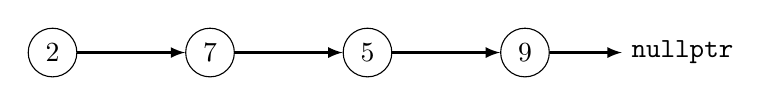
\begin{tikzpicture}
			[every circle node/.style={draw}]
			\node[circle] (A) at (0,0) {2};
			\node[circle] (B) at (2,0) {7};
			\node[circle] (C) at (4,0) {5};
			\node[circle] (D) at (6,0) {9};
			\node (E) at (8,0) {\texttt{nullptr}};
			\path[-latex,draw,thick]
			(A) edge (B)
			(B) edge (C)
			(C) edge (D)
			(D) edge (E);
		\end{tikzpicture}
		\item Doubly linked list: can be traversed backwards\\
		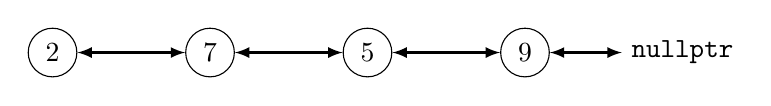
\begin{tikzpicture}
			[every circle node/.style={draw}]
			\node[circle] (A) at (0,0) {2};
			\node[circle] (B) at (2,0) {7};
			\node[circle] (C) at (4,0) {5};
			\node[circle] (D) at (6,0) {9};
			\node (E) at (8,0) {\texttt{nullptr}};
			\path[latex-latex,draw,thick]
			(A) edge (B)
			(B) edge (C)
			(C) edge (D)
			(D) edge (E);
		\end{tikzpicture}
		\item Circular linked list:\\
		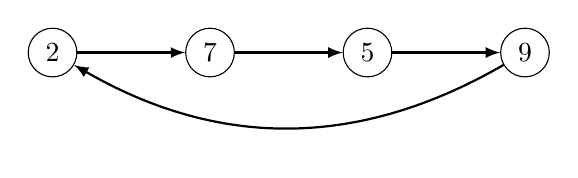
\begin{tikzpicture}
			[every circle node/.style={draw}]
			\node[circle] (A) at (0,0) {2};
			\node[circle] (B) at (2,0) {7};
			\node[circle] (C) at (4,0) {5};
			\node[circle] (D) at (6,0) {9};
			\path[-latex,draw,thick]
			(A) edge (B)
			(B) edge (C)
			(C) edge (D)
			(D) edge[bend left] (A);
		\end{tikzpicture}
		\item Circular doubly linked list:\\
		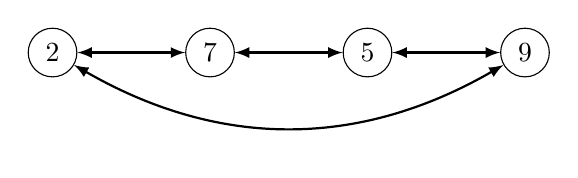
\begin{tikzpicture}
			[every circle node/.style={draw}]
			\node[circle] (A) at (0,0) {2};
			\node[circle] (B) at (2,0) {7};
			\node[circle] (C) at (4,0) {5};
			\node[circle] (D) at (6,0) {9};
			\path[latex-latex,draw,thick]
			(A) edge (B)
			(B) edge (C)
			(C) edge (D)
			(D) edge[bend left] (A);
		\end{tikzpicture}
	\end{itemize}
	\item Basic operations' complexity:
	\begin{center}
		\begin{tabular}{|l|c|c|}
			\hline
			& Singly Linked List & Doubly Linked List \\ \hline
			Search & $ \color{Orange} \mathcal{O}(N) $ & $ \color{Orange} \mathcal{O}(N) $ \\ \hline
			Insert at head & $ \color{Green} \mathcal{O}(1) $ & $ \color{Green} \mathcal{O}(1) $ \\ \hline
			Insert at tail & $ \color{Green} \mathcal{O}(1) $ & $ \color{Green} \mathcal{O}(1) $ \\ \hline
			Delete at head & $ \color{Green} \mathcal{O}(1) $ & $ \color{Green} \mathcal{O}(1) $ \\ \hline
			Delete at tail & $ \color{Orange} \mathcal{O}(N) $ & $ \color{Green} \mathcal{O}(1) $ \\ \hline
			Delete at middle & $ \color{Orange} \mathcal{O}(N) $ & $ \color{Orange} \mathcal{O}(N) $ \\ \hline
		\end{tabular}
	\end{center}
	\item Implementation in \texttt{C++}: \texttt{std::list} and \texttt{std::forward\_list}
\end{itemize}

A (too) simple draft in \texttt{C++} for doubly linked list:
\begin{lstlisting}[language=C++]
template<typename T>
struct Node
{
	T val_;
	Node<T> *prev_, *next_;
};

template<typename T>
struct DoublyLinkedList
{
	Node<T> head_, tail_;
	int size_;
	
	void clear();
	void insert(const T &val, const T &prev_val);
	void remove(const T &val);
}
\end{lstlisting}

Less common operations:
\begin{itemize}
	\item Swap nodes without swapping data: simply search for the two nodes.\\
	Can be optimized a bit by running 1 single traverse instead of 2, time complexity $\mathcal{O}(N)$
	\item Rotate a Linked List: by placing the first element at the end.
	\item Reverse a Linked List: time complexity $\mathcal{O}(N)$
	\begin{itemize}
		\item Divide the list in two parts – first node and rest of the linked list.
		\item Call reverse for the rest of the linked list.
		\item Link the rest linked list to first.
		\item Fix head pointer to \texttt{nullptr}
	\end{itemize}
	\item Merge two sorted linked lists: time complexity $\mathcal{O}(M + N)$ (sizes of two lists)
	\begin{itemize}
		\item Create a dummy node for the merged list and two pointers for traversing two lists
		\item Traverse the lists until reaching the end \texttt{nullptr}
		\item While traversing, compare the node values of the pointers
	\end{itemize}
	\item Merge Sort for linked lists: time complexity $\mathcal{O}(N)$, memory complexity $\mathcal{O}(N)$ or $\mathcal{O}(\log N)$
	\begin{itemize}
		\item If the \texttt{head\_ptr} is \texttt{nullptr} or there is only 1 element, then \texttt{return}
		\item Else divide the list into two halves
		\item Sort the two halves
		\item Merge the two sorted linked lists (check above)
	\end{itemize}
	\item Reverse a Linked List in groups of given size??
	\item Detect and Remove Loop in a Linked List
\end{itemize}

\section{Stack}

\begin{itemize}
	\item \ac{ADT} for \ac{LIFO}
	\item Basic operations
	\begin{itemize}
		\item Push: append new elements
		\item Pop: remove the top element
		\item Peek: view the top element without popping it from the stack
	\end{itemize}
	\item Complexity
	\begin{center}
		\begin{tabular}{|l|c|}
			\hline
			Pushing & $ \color{Green} \mathcal{O}(1) $ \\ \hline
			Popping & $ \color{Green} \mathcal{O}(1) $ \\ \hline
			Peeking & $ \color{Green} \mathcal{O}(1) $ \\ \hline
			Searching & $ \color{Orange} \mathcal{O}(N) $ \\ \hline
			Size & $ \color{Green} \mathcal{O}(1) $ \\ \hline
		\end{tabular}
	\end{center}
	\item Implementation: \texttt{std} library, using linked lists, \etc
	\item Usage
	\begin{itemize}
		\item Used behind the scene to support recursion
		\item Find the next greater element \href{https://www.geeksforgeeks.org/next-greater-element/}{\texttt{(geeksforgeeks.org)}}
		\item Can be used to do Depth First Search
		\item Balanced parenthesis
		\item Backtracking
		\item Reverse a word, vector, \etc
	\end{itemize}
\end{itemize}

\section{Queue}
\begin{itemize}
	\item Is a linear data structure which models real world queues for \ac{FIFO}
	\item Two primary operations, \ie, enqueue and dequeue.
	\item Complexity
	\begin{center}
		\begin{tabular}{|l|c|}
			\hline
			Enqueue & $ \color{Green} \mathcal{O}(1) $ \\ \hline
			Dequeue & $ \color{Green} \mathcal{O}(1) $ \\ \hline
			Peeking & $ \color{Green} \mathcal{O}(1) $ \\ \hline
			Contains & $ \color{Orange} \mathcal{O}(N) $ \\ \hline
			Removal & $ \color{Orange} \mathcal{O}(N) $ \\ \hline
			Is empty & $ \color{Green} \mathcal{O}(1) $ \\ \hline
		\end{tabular}
	\end{center}
	\item Usage:
	\begin{itemize}
		\item Breadth first search
		\item Task scheduling: CPU, disk management, data transfer. 
		\item Find the starting node for a circular traverse over a graph \href{https://www.geeksforgeeks.org/find-a-tour-that-visits-all-stations/}{\texttt{(geeksforgeeks.org)}}
		\item \etc
	\end{itemize}
	\item Implementation:
	\begin{itemize}
		\item Array
		\item (Singly / Doubly) Linked list: enqueueing is adding elements to the tail, dequeueing is delete elements at the head
	\end{itemize}
\end{itemize}

\section{Priority Queue}
\begin{itemize}
	\item Priority Queue is an \ac{ADT}, similar to normal queue, except that each element has a priority score.
	\item Usage:
	\begin{itemize}
		\item Dijkstra's algorithm
		\item Best First Search algorithm: \eg, A* algorithm
		\item Minimum Spanning Tree
	\end{itemize}
	\item Complexity
	\begin{center}
		\begin{tabular}{|l|l|}
			\hline
			Binary Heap construction & $ \color{Red} \mathcal{O}(N) $ \\ \hline
			Polling & $ \color{Orange} \mathcal{O}(\log N) $ \\ \hline
			Peeking & $ \color{Green} \mathcal{O}(1) $ \\ \hline
			Adding & $ \color{Orange} \mathcal{O}(\log N) $ \\ \hline
			Naive removing & $ \color{Red} \mathcal{O}(N) $ \\ \hline
			Removing with hash table & $ \color{Orange} \mathcal{O}(\log N) $ \\ \hline
			Naive contains & $ \color{Red} \mathcal{O}(N) $ \\ \hline
			Contains with hash table & $ \color{Green} \mathcal{O}(1) $ \\ \hline
		\end{tabular}
	\end{center}
	\item Turning Min PQ to Max PQ: simply by subtracting the maximum score
\end{itemize}

\section{Heap}
\begin{itemize}
	\item Is one common implementation for Priority Queue
	\item Is a \ac{DS} that satisfies the \textit{\textbf{heap invariant}}
	\item Types of heaps:
	\begin{itemize}
		\item Binary heap: a binary tree that supports the \textbf{\textit{heap invariant}}
		\item Fibonacci heap
		\item Binomial heap
		\item Pairing heap
	\end{itemize}
	\item Adding element to gradually form a complete binary tree: by simply bubbling up if it violates the \textbf{\textit{heap invariant}}
	\item Polling / Removing the top element:
	\begin{itemize}
		\item Swap it with the last element in the array
		\item Delete it (at the last position)
		\item The element at top violates the heap invariant, bubbling it down, swap with the smallest child nodes
		\item If they are tie, go for the left one
	\end{itemize}
	\item Removing specific element:
	\begin{itemize}
		\item Find that element in linear time
		\item Swap it with the last element and remove it
		\item Bubbling up or down to satisfy the heap invariant
	\end{itemize}
\end{itemize}

\section{Union}

Union Find, or Disjoint Set:
\begin{itemize}
	\item Is a \ac{DS} that keeps track of elements which are split into one or more disjoint sets
	\item Primary operations: find and union
	\begin{itemize}
		\item Find: which component/set a particular element belongs to
		\item Union: unify two elements, by make the root of one point to the other root
	\end{itemize}
	\item Usage
	\begin{itemize}
		\item Kruskal's minimum spanning tree algorithm
		\item Grid percolation
		\item Network connectivity
		\item Least common ancestor in trees
		\item Image processing
	\end{itemize}
	\item Complexity:
	\begin{center}
		\begin{tabular}{|l|l|}
			\hline
			Construction & $ \color{Red} \mathcal{O}(N) $ \\ \hline
			Union & $ \color{Orange} \alpha(N) $ \\ \hline
			Find & $ \color{Orange} \alpha(N) $ \\ \hline
			Get component size & $ \color{Orange} \alpha(N) $ \\ \hline
			Check if connected & $ \color{Orange} \alpha(N) $ \\ \hline
			Count components & $ \color{Green} \mathcal{O}(1) $ \\ \hline
		\end{tabular}
	\end{center}
	\item Construct a bijection (mapping) between your objects and the integers in the range $ [0, n) $ (not necessary, but recommended)
	\begin{itemize}
		\item In the array, each position is for an object
		\item The value in each position is the root node of that object. Initially, the root of an object is itself
		\item As the objects are grouped together, the root of each object will changed.
		\item Also keep an array of the size of each group so we can break the tie if necessary, or return the size of the group
		\item Path compression: when taking union, not only point the old root to the new root, but also point all elements of the old/smaller set to the new root.
	\end{itemize}
\end{itemize}

\section{Binary Search Tree}
\begin{itemize}
	\item Basic definitions:
	\begin{itemize}
		\item Tree is an undirected graph / acyclic connected graph, has N nodes and N-1 edges
		\item Root node, child, parent node, leaf node, subtree
		\item Binary tree is a tree for which every node has at most two child nodes
		\item \ac{BST} is a binary tree that satisfies \ac{BST} invariant: left subtree has smaller elements, and right subtree has larger elements (possibly when comparing with the root node)
	\end{itemize}
	\item Usage: Implementation of some map and set \ac{ADT}s, red black trees, AVL trees, splay trees, binary heaps, syntax trees, \etc
	\item Complexity:
	\begin{center}
		\begin{tabular}{|l|c|c|}
			\hline
			Operation & Average & Worst \\ \hline
			Insert & $ \color{Orange} \mathcal{O}(\log N) $ & $ \color{Red} \mathcal{O}(N) $\\ \hline
			Delete & $ \color{Orange} \mathcal{O}(\log N) $ & $ \color{Red} \mathcal{O}(N) $\\ \hline
			Remove & $ \color{Orange} \mathcal{O}(\log N) $ & $ \color{Red} \mathcal{O}(N) $\\ \hline
			Search & $ \color{Orange} \mathcal{O}(\log N) $ & $ \color{Red} \mathcal{O}(N) $\\ \hline
		\end{tabular}
	\end{center}
	Balanced binary search trees were invented due to bad linear behavior in the worst case.
\end{itemize}

Operation in \ac{BST}: Elements must be \hlb{comparable}
\begin{itemize}
	\item Insertion: compare the element to current node, recurse down accordingly
	\item Removal: find the element (if exists), replace the node with its child node to maintain the \ac{BST} invariant
	\begin{itemize}
		\item If leaf node, remove it
		\item If has just one left or right subtree, replace the node with the subtree
		\item If has both subtree, either replace with largest node in the left subtree or smallest node in the right subtree
	\end{itemize}
	\item Traversal:
\begin{lstlisting}[language=C++]
void preorder(node) {
	if (node == nullptr) return;
	print(node.value);
	preorder(node.left);
	preorder(node.right);
}

void inorder(node) {
	if (node == nullptr) return;
	inorder(node.left);
	print(node.value);
	inorder(node.right);
}

void postorder(node) {
	if (node == nullptr) return;
	postorder(node.left);
	postorder(node.right);
	print(node.value);
}
\end{lstlisting}
	\item level-order traversal: \ac{BFS} with queue
\end{itemize}

\section{Hash Table}
\begin{itemize}
	\item A Hash table is a data structure mapping keys to values using hash functions.
	\item Keys must be unique, but values can be repeated
	\item Usage
	\begin{itemize}
		\item Track item frequencies
	\end{itemize}
	\item Properties of hash functions:
	\begin{itemize}
		\item If $ H(x) = H(y) $, then objects $ x $ and $ y $ might be equal
		\item If $ H(x) \neq H(y) $, then objects $ x $ and $ y $ are certainly not equal
		\item A Hash function must be deterministic
		\item We try very hard to make uniform hash functions to minimize the number of hash collisions
	\end{itemize}
	\item The hash function is used as a way to index into the array, which is the hash table.
	\item Dealing with hash collision
	\begin{itemize}
		\item Separate chaining: maintaining a data structure (usually a linked list) to hold all the different values which hashed to a particular value
		\item Open addressing: finding another place within the hash table for the object to go by offsetting it from the position to which it hashed to
	\end{itemize}
	\item Complexity:
	\begin{center}
		\begin{tabular}{|l|c|c|}
			\hline
			Operation & Average & Worst \\ \hline
			Insertion & $ \color{Green} \mathcal{O}(1) $* & $ \color{Red} \mathcal{O}(N) $\\ \hline
			Removal & $ \color{Green} \mathcal{O}(1) $* & $ \color{Red} \mathcal{O}(N) $\\ \hline
			Search & $ \color{Green} \mathcal{O}(1) $* & $ \color{Red} \mathcal{O}(N) $\\ \hline
		\end{tabular}
	\end{center}
\end{itemize}

\section{Fenwick Tree}
Fenwick Tree, \ac{aka}, Binary Indexed Tree
\begin{itemize}
	\item A \ac{DS} that supports sum range queries as well as setting values in a static array
	\item Complexity:
	\begin{center}
		\begin{tabular}{|l|c|}
			\hline
			Construction & $ \color{Orange} \mathcal{O}(N) $ \\ \hline
			Point Update & $ \color{Green} \mathcal{O} (\log N) $ \\ \hline
			Range Sum & $ \color{Green} \mathcal{O} (\log N) $ \\ \hline
			Range Update & $ \color{Green} \mathcal{O} (\log N) $ \\ \hline
			Adding Index & \color{Red} $ N/A $ \\ \hline
			Removing Index & \color{Red} $ N/A $ \\ \hline
		\end{tabular}
	\end{center}
	\item The tree and array is base 1, not 0
	\item Each element/node in the tree is responsible for a specific range
	\begin{figure}[hbt!]
		\centering
		\includegraphics[width=0.2\textwidth]{fenwick-tree.png}
		\caption{Fenwick tree: each node is responsible for a specific (blue) range}
	\end{figure}
\end{itemize}

\section{Balanced Binary Search Tree}
\begin{itemize}
	\item \ac{BBST} is a self-balanced \ac{BST}
	\item \ac{BBST} adjusts itself in order to maintain a low (logarithmic) height allowing for faster operations such as insertions and deletions
	\item Complexity: unlike \ac{BST}, \ac{BBST}'s time complexity for all tasks (insert, delete, remove, search) is $ \color{Orange} \mathcal{O}(\log N) $
	\item Tree invariant is property/rule that the tree must satisfy after every operation. If not, rotations are applied
	\item Tree rotations
\begin{lstlisting}[language=C++]
void rightRotate(Node* node) {
	
	Node* P = A->parent;
	Node* B = A->left;
	A->left = B->right;
	B->right = A;
	// Also change pointer of A's parent
}
\end{lstlisting}
	\item AVL tree is one of many types of \ac{BBST}, \eg, 2-3 tree, the AA tree, the scapegoat tree, red-black tree
\end{itemize}

\section{Segment Tree}
\begin{itemize}
	\item Read \href{https://cp-algorithms.com/data_structures/segment_tree.html}{cp-algorithms}
	\item A \ac{DS} that stores information about array intervals as a tree
	\item It allows range queries and point update over an array efficiently
	\begin{center}
		\begin{tabular}{|l|c|}
			\hline
			Point Update & $ \color{Green} \mathcal{O} (\log N) $ \\ \hline
			Range Query & $ \color{Green} \mathcal{O} (\log N) $ \\ \hline
		\end{tabular}
	\end{center}
	As the height of the tree is $ \mathcal{O} (\log N) $
	\item The standard Segment tree requires $ 4N $ vertices for working on an array of size $ N $
	\item Just as in a binary tree, with the \texttt{ID\_P} of the parent node, the \texttt{ID} of child nodes can be easily identified: \texttt{(ID\_P * 2 + 1)} and \texttt{(ID\_P * 2 + 2)}
	\item Check the source code for implementation details
\end{itemize}

\begin{figure}[hbt!]
	\centering
	\includegraphics[width=0.7\textwidth]{segment-tree.png}
	\caption{Segment tree for sum queries}
\end{figure}

\section{Sparse Table}
\begin{itemize}
	\item Check: \href{https://youtu.be/uUatD9AudXo}{WilliamFiset}
	\item Sparse Table is all about doing efficient \hlb{range queries} on a static / \hlb{immutable array}
	\item The high level idea in sparse table is simply to pre-computed the answer for all possible range queries of size $ 2^x $ (\figref{fig:sparse-table})
	\begin{figure}[hbt!]
		\centering
		\includegraphics[width=0.7\textwidth]{sparse-table.png}
		\caption{Example of sparse table with $ \min $ query. Each cell is responsible to answer a range of size $ 2^x $}
		\label{fig:sparse-table}
	\end{figure}
	\item Common type queries: min, max, sum, gcd, \etc
	\item The table can be filled using dynamic programming
	\begin{align*}
		dp[i][j] & = f(dp[i-1][j], dp[i-1][j+2^{i-1}]) \\
		& = \min(dp[i-1][j], dp[i-1][j+2^{i-1}]) \\
		dp[3][2] & = \min(dp[2][2], dp[2][2 + 2^{3-1}]) = \min(dp[2][2], dp[2][6])
	\end{align*}
	\item If the query is based on an associative functions, sparse table can answer in $ \mathcal{O} (\log_2 N) $\\
	$ f(a, f(b, c)) = f(f(a, b), c) \quad\forall a, b, c$. \Eg: sum, product, \etc
	\item If the query is based on an \textit{"overlap friendly"} functions, we will reach constant time $ \mathcal{O} (1) $\\
	$ f(f(a, b), f(b, c)) = f(f(a, b), c) = f(a, f(b, c)) $. \Eg: min, max, gcd, \etc\\
	Thus: $ f(l, r) = f(f(l, k), f(k+1, r)) $\\
	\Eg: for $ \min[2,7] $, calculate $ p = floor(\log_2(7-2+1)) = 2 $; $ k = 2^p = 4 $\\
	$\Rightarrow$ $ min[2, 7] = \min(t[2][2], t[2][4]) $
	\item If the function is not overlap agnostic, we have to break down the range quite similar to in a segment tree in $ \mathcal{O} (\log_2 N) $\\
	\Eg: with product query: $ prod[0, 6] = t[2][0] * t[1][4] * t[0][6] $
\end{itemize}

\section{Suffix Array}
\begin{itemize}
	\item References: \href{https://codeforces.com/edu/course/2/lesson/2/1}{codeforces}
	\item The suffix array is an array containing all the sorted suffixes of a string
	\item It is actually the array of sorted indices of the suffixes
	\item The suffix array and \hlb{suffix tree} are different, but both are compressed version of a \hlb{trie}
	\item Usage:
	\begin{itemize}
		\item The Longest Common Prefix (LCP) array
	\end{itemize}
\end{itemize}

\section{Graph}

\section{Matrix}

\section{Advanced Data Structure}